\section{Tecnologie}
\subsection{Python}
Il linguaggio di programmazione utilizzato per perseguire gli obiettivi del progetto è stato Python\textit{v3.7}, si tratta di un linguaggio di programmazione di alto livello il cui obiettivo è quello di facilitare la leggibilità del codice ed adattarsi a diversi paradigmi di programmazione come quello procedurale, ad oggetti e funzionale. La motivazione per la scelta dell'utilizzo di questo linguaggio, oltre alla sua semplicità, è per il suo supporto di numeri frameworks e moduli relativi al deep learning e alla computer vision tra i quali Tensorflow e OpenCV. Qualsiasi modulo aggiuntivo può essere semplicemente installato eseguendo il comando:
\begin{verbatim}
pip install nome_modulo
\end{verbatim}
Per lanciare un programma viene utilizzato il comando:
\begin{verbatim}
python nome_file.py
\end{verbatim}
Altri moduli che sono stati utilizzati comprendono Numpy, Matplotlib e Pytest.
\begin{figure}[H]
	\centering
	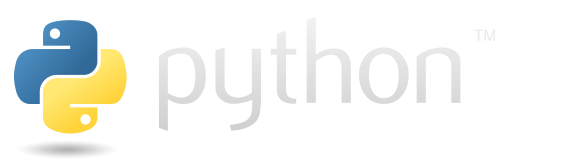
\includegraphics[width=0.7\linewidth]{images/logo-python.png}
	\caption{Logo di Python}
	\label{Logo di Python}
\end{figure}
\subsection{Pycharm}
Pycharm è un IDE per programmare in Python sviluppato da JetBrains. Le sue caratteristiche più importanti includono: 
\begin{itemize}
\item Un sistema intelligente di completamento automatico del codice;
\item Analisi statica del codice eseguita a tempo di esecuzione;
\item Individuazione e risoluzione veloce degli errori tramite proposte di correzione;
\item Possibilità di lavorare in un ambiente di sviluppo virtuale dove per ogni progetto vengono installate solamente le proprie dipendenze ed i propri moduli. 
\end{itemize}
\subsection{Tensorflow}
Tensorflow\cite{tensorflow} è un framework gratuito e open-source per lo sviluppo e l'allenamento di modelli di machine learning come le reti neurali. Ha la particolarità che i dati vengono gestiti attraverso dei grafi computazionali dove i nodi rappresentano delle operazioni matematiche da eseguire e gli archi rappresentano degli array multidimensionali contenenti i dati sui quali svolgere le operazioni (tensori). La sua architettura permette di svolgere le operazioni sia usando le CPUs che le GPUs in modo da eseguire operazioni con alto livello di parallelismo. Il modello di rete neurale utilizzato per effettuare la detection sulle immagini è stato implementato con Tensorflow.
\begin{figure}[H]
	\centering
	
\includegraphics[width=0.3\linewidth]{images/logo-tensorflow.png}
	\caption{Logo di Tensorflow}
	\label{Logo di Tensorflow}
\end{figure}
\subsection{OpenCV}
OpenCV\cite{opencv} è una libreria open-source orientata allo sviluppo di applicazioni di computer vision in tempo reale. E' stata scritta originariamente in C++ ma offre anche il supporto ad altri linguaggi di programmazione come Python. OpenCV è un' ottima libreria quando si ha bisogno di manipolare immagini e video permettendo di compiere operazioni sia di alto livello che di basso livello operando sui singoli pixels. Sono inoltre presenti diversi algoritmi di object detection ed object tracking già implementati permettendo quindi di sperimentarli tutti senza apportare troppe modifiche al proprio programma. La libreria è stata anche utilizzata per scomporre un video nei sui singoli frames oltre che per disegnare su di essi.
\subsection{Numpy}
Numpy\cite{numpy} è un modulo di Python che fornisce il supporto per la gestione di matrici e array multidimensionali di grandi dimensioni. Dispone anche di una vasta collezione funzioni matematiche per lavorare ad alto livello su di essi. Viene spesso utilizzato per operare su grandi quantità di dati in modo rapido ed efficiente.
\subsection{Matplotlib}
Matplotlib\cite{matplotlib} è una libreria grafica sviluppata per Python impiegata principalmente per disegnare grafici o altre figure con lo scopo di rappresentare dei dati utilizzando il minor numero di righe di codice possibile. In fase di allenamento di una rete neurale viene spesso usato per mostrare l'andamento della variazione dell'errore e dell'accuratezza della rete.
\subsection{Pytest}
Pytest\cite{pytest} è un framework per Python che permettere di scrivere dei test per testare il codice permettendone la loro esecuzione in modo automatico. Per installarlo viene utilizzato il comando:
\begin{verbatim}
pip install pytest
\end{verbatim}
mentre per lanciarne l'esecuzione viene usato il comando:
\begin{verbatim}
pytest nome_file
\end{verbatim}
Per convenzione il file contenente i test relativi ad un solo modulo è stato chiamato "nome\_modulo\_test.py" dove "nome\_modulo.py" è il modulo ad esso associato. I metodi che eseguono un test devono iniziare con "test\_", in caso contrario non verranno riconosciuti come tali e la loro esecuzione non verrà lanciata. Sono stati implementati dei test di unità per tutte le funzioni più complesse o critiche in modo da verificarne il corretto funzionamento. Sono anche stati sviluppati dei test di integrazione per ogni algoritmo implementato in modo da assicurarsi del loro corretto funzionamento. Per valutare l'esecuzione dell'intero sistema sono invece state utilizzate delle metriche per misurare la bontà del risultato in quanto i test di sistema non sarebbero stati adatti per misurare un risultato non deterministico come il riconoscimento di oggetti o la qualità del tracking.
\subsection{Excel}
Il foglio elettronico Excel si è rivelato molto utile nel visualizzare ed ordinare grandi quantità di dati. In particolare, i risultati ottenuti eseguendo le detections sono stati automaticamente collezionati e raggruppati in un foglio elettronico tramite un script in Python ai fini di agevolare il loro ordinamento e permettere una rapida selezione dei risultati migliori.
